\clearpage
\begin{appendices}

% ------------------------------------------------------------------------------

% první příloha
\priloha{Osudový dopis A.~Autora}

\textit{
Textová příloha může být příkladem přepisu korespondence mezi slavnými
skladateli, o~které je pojednáváno ve~vlastním textu práce.
}

\noindent
Vážený A. Autore,

\lipsum

\lipsum

\begin{flushright}
Se srdečným pozdravem \\
C.D. Skladatel
\end{flushright}

% ------------------------------------------------------------------------------

% druhá příloha
\priloha{Vložená partitura}

\begin{figure}[!ht]
	\begin{center}
		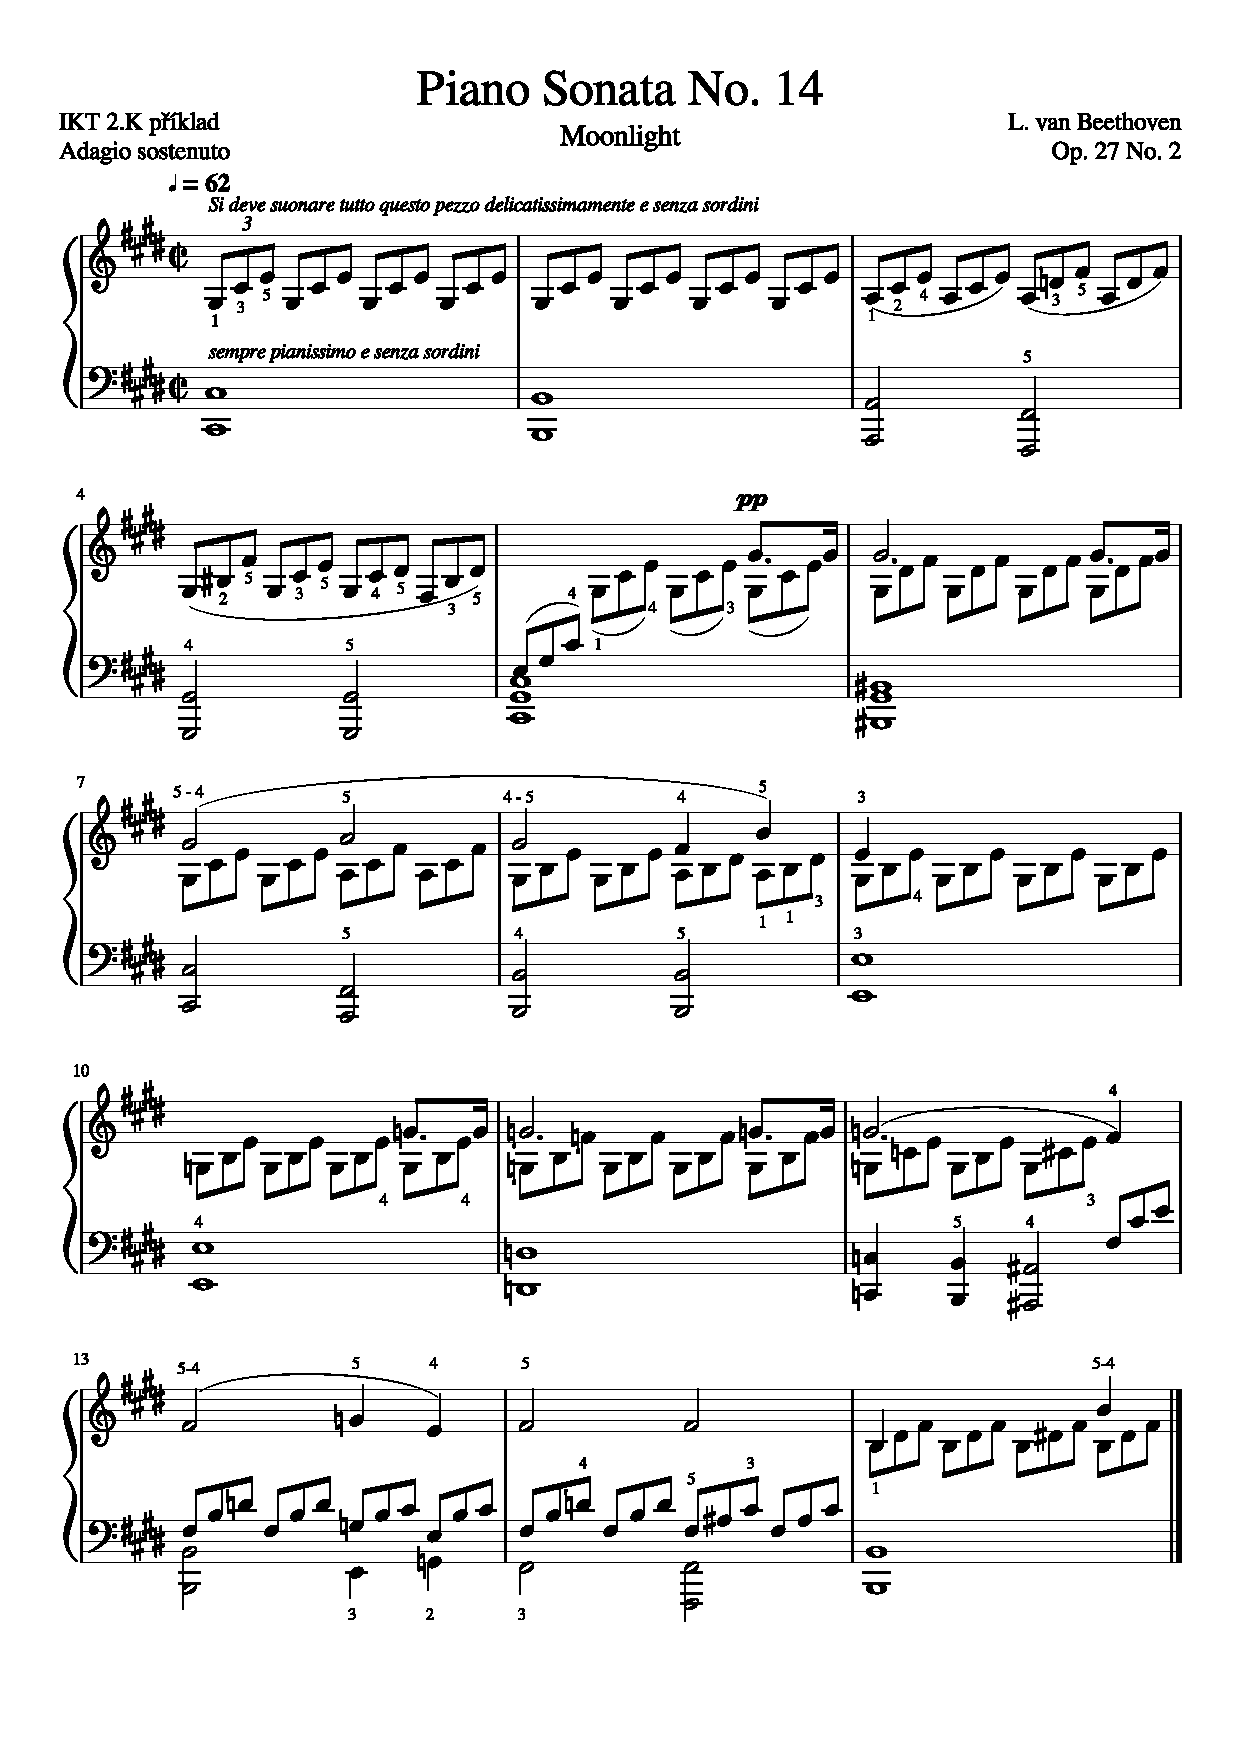
\includegraphics[width=\textwidth]{./obrazky/partitura-priklad.pdf}
    \end{center}
\end{figure}

\noindent
Přiložená partitura je příkladem naskenovaného notového materiálu o~výšce
větší než polovina stránky, o~kterém je pojednáváno ve~vlastním textu práce.

% ------------------------------------------------------------------------------

\end{appendices}
